\textbf{Prerequisites}\\

A computer with an NVIDIA graphics card that is CUDA compatible (RTX 2070 was used in this study). Although you can train with a CPU, it will be significantly slower.\\
A virtual environment with Python 3.8 – 3.11 (Python 3.9.16 was used in this study).

\begin{figure}[H]
    \centering
    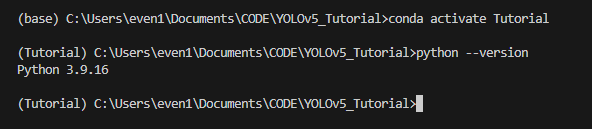
\includegraphics[scale=0.5]{evenbilder/tutorial/tutorial-1.png}
    \label{fig:tutorial-1}
\end{figure}

1.	Install Pytorch: Start by installing the correct version of Pytorch. Visit Pytorch's website and select the version that suits your hardware. If your GPU supports CUDA, select "compute platform" CUDA 11.8. If your GPU is not supported, opt for the CPU version.\\

\begin{figure}[H]
    \centering
    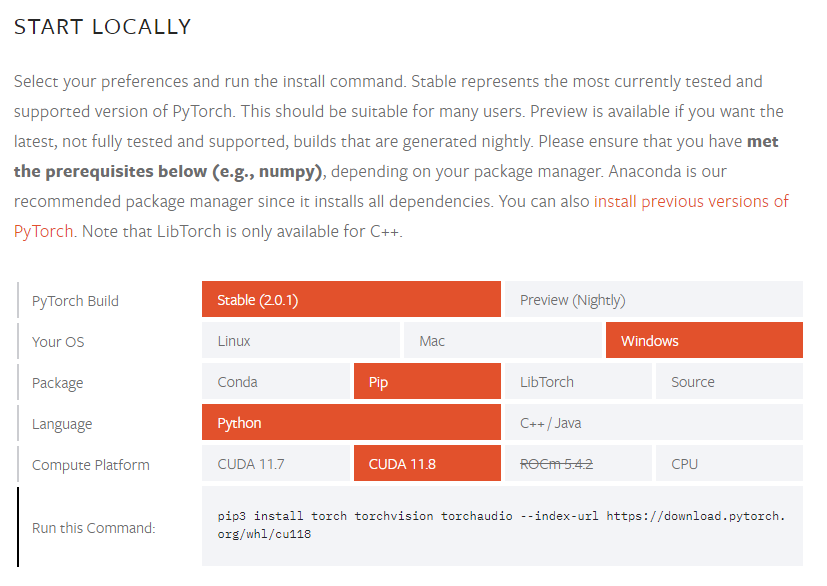
\includegraphics[scale=0.5]{evenbilder/tutorial/tutorial-2.png}
    \label{fig:tutorial-2}
\end{figure}

2.	Run the Pytorch Command: Execute the provided command in your Python environment. This might take some time, as Pytorch will download and install all necessary packages.\\

\begin{figure}[H]
    \centering
    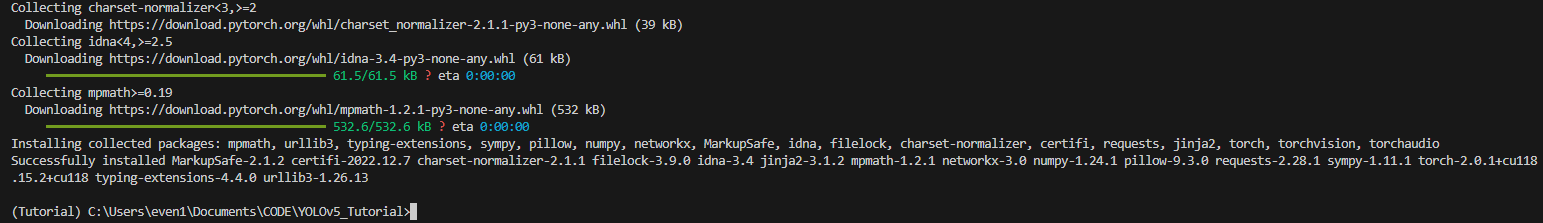
\includegraphics[scale=0.5]{evenbilder/tutorial/tutorial-3.png}
    \label{fig:tutorial-3}
\end{figure}
\newpage
3.	Download and Install the Correct CUDA Version.\\

\begin{figure}[H]
    \centering
    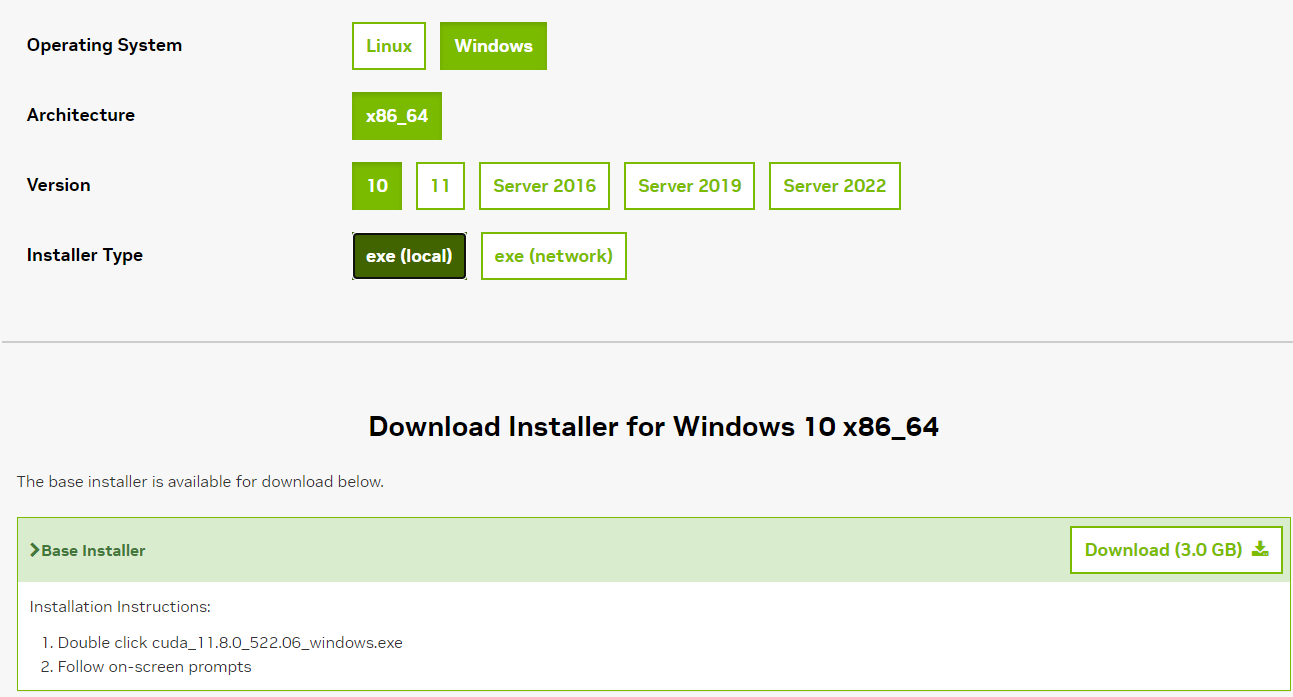
\includegraphics[scale=0.5]{evenbilder/tutorial/tutorial-4.png}
    \label{fig:tutorial-4}
\end{figure}

4.	Verify CUDA Installation: Follow the steps in the installer. After installation, use the command nvcc --version to ensure that CUDA has been installed correctly.\\

\begin{figure}[H]
    \centering
    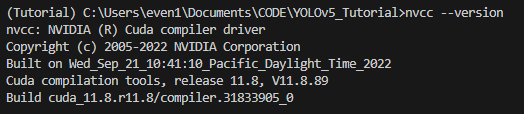
\includegraphics[scale=0.5]{evenbilder/tutorial/tutorial-5.png}
    \label{fig:tutorial-5}
\end{figure}

5.	Clone the YOLO Repository and Install Requirements.\\

git clone https://github.com/ultralytics/yolov5  \\
cd yolov5\\
pip install -r requirements.txt  \\

6.	We recommend running the following script once to train on the COCO dataset, as this will create the correct folder structure and download the necessary weights: python train.py --img 640 --epochs 3 --data coco128.yaml --weights yolov5n.pt\\

\begin{figure}[H]
    \centering
    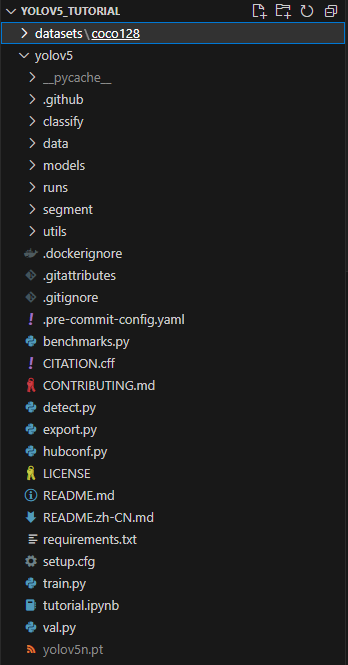
\includegraphics[scale=0.5]{evenbilder/tutorial/tutorial-6.png}
    \label{fig:tutorial-6}
\end{figure}

7.	Duplicate and Rename the YAML File: Make a copy of the coco128.yaml file found under yolov5/data/ and rename it to match your dataset. This file instructs the training command where to find the dataset and corresponding labels.\\

\begin{figure}[H]
    \centering
    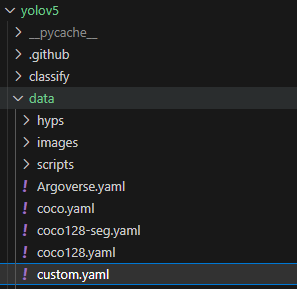
\includegraphics[scale=0.5]{evenbilder/tutorial/tutorial-7.png}
    \label{fig:tutorial-7}
\end{figure}

8.	Modify the YAML File: Adjust the file to meet your requirements. For instance, in this study, we only have one class, named "greenball".\\

\begin{figure}[H]
    \centering
    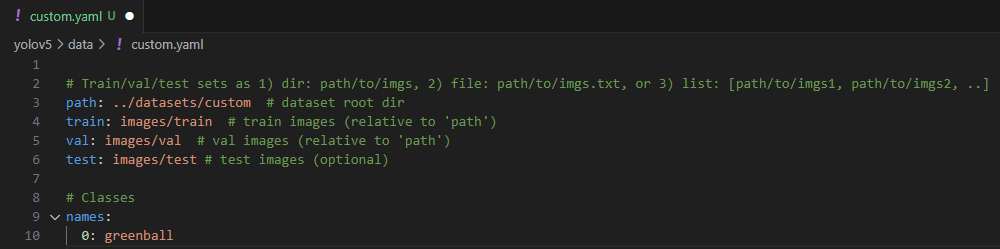
\includegraphics[scale=0.5]{evenbilder/tutorial/tutorial-8.png}
    \label{fig:tutorial-8}
\end{figure}

10.	You're now ready to begin training your YOLO model on your custom data. Decide on the model you want to use for transfer learning. We recommend either yolov5n (nano) or yolov5s (small), as larger models result in slower frame rates.\\

python train.py --img 640 --epochs 3 --data custom.yaml --weights yolov5n.pt --device 0\\

Ensure that the YAML file selected is the custom one you created earlier. \\

Choose the number of epochs for training; a range of 500 to 1000 is recommended. 
The img 640 parameter determines the size to which the image is scaled (640 is YOLO's default).\\ 
To execute the process on CPU, remove the --device 0 parameter.\\

11.	Examine Training Results: Upon completion of training, you'll find all related materials saved under the runs/train/ directory. The most recent training session will be in the latest exp folder. This folder contains the retrained weights and general statistics from the training process, including plots that visualize the training progress.\\

\begin{figure}[H]
    \centering
    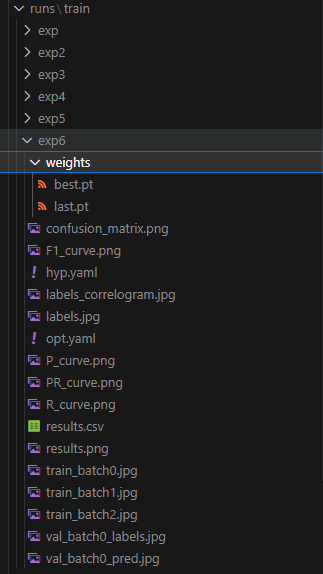
\includegraphics[scale=0.5]{evenbilder/tutorial/tutorial-10.png}
    \label{fig:tutorial-10}
\end{figure}

12. After successfully training your YOLO model, you can test it in real-time using your webcam. Run the following command:\\

python detect.py --weights <path to weights> --source 0

Replace <path to weights> with the path to your trained weights file. The --source 0 specifies that the webcam (usually denoted by '0' in most systems) should be used as the input source.